\noindent\makebox[0pt][r]{%
  \makebox[44mm][l]{\textsf{\textbf{282}}}\hspace{6mm}%
}%
\textsf{\textbf{CHƯƠNG 4}}\hspace{1.5em}\textsf{Các ứng dụng của đạo hàm}
\vspace{1.2em}

Các Hình 9 và 10 cho thấy một hàm số không nhất thiết phải có các giá trị cực trị nếu một trong hai giả thiết (tính liên tục hoặc đoạn đóng) bị lược bỏ khỏi Định lý Giá trị Cực trị.

\vspace{0.6em}
\noindent
\begin{minipage}[t]{0.48\textwidth}
  \centering
  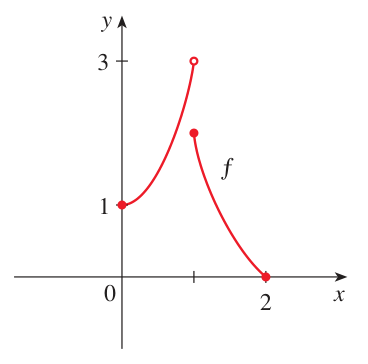
\includegraphics[width=0.88\linewidth]{images/p0317_fig1.png}\\[4pt]
  \raggedright
  {\small\textbf{\textsf{HÌNH 9}}\\[1pt]
  Hàm số này có giá trị nhỏ nhất $f(2) = 0$, nhưng không có giá trị lớn nhất.}
\end{minipage}\hfill
\begin{minipage}[t]{0.48\textwidth}
  \centering
  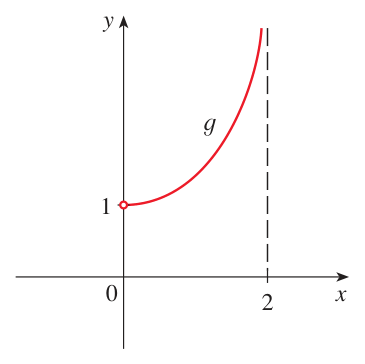
\includegraphics[width=0.88\linewidth]{images/p0317_fig2.png}\\[4pt]
  \raggedright
  {\small\textbf{\textsf{HÌNH 10}}\\[1pt]
  Hàm số liên tục $g$ này không có giá trị lớn nhất hoặc nhỏ nhất.}
\end{minipage}

\vspace{0.8em}
Hàm số $f$ có đồ thị trong Hình 9 được xác định trên đoạn đóng $[0, 2]$ nhưng không có giá trị lớn nhất. (Lưu ý rằng tập giá trị của $f$ là $[0, 3)$. Hàm số nhận các giá trị gần 3 tùy ý, nhưng không bao giờ thực sự đạt tới giá trị 3.) Điều này không mâu thuẫn với Định lý Giá trị Cực trị vì $f$ không liên tục. [Tuy nhiên, một hàm số gián đoạn \emph{vẫn có thể} có các giá trị lớn nhất và nhỏ nhất. Xem Bài tập 13(b).]

Hàm số $g$ trong Hình 10 liên tục trên khoảng mở $(0, 2)$ nhưng không có giá trị lớn nhất lẫn giá trị nhỏ nhất. [Tập giá trị của $g$ là $(1, \infty)$. Hàm số nhận các giá trị lớn tùy ý.] Điều này không mâu thuẫn với Định lý Giá trị Cực trị vì khoảng $(0, 2)$ không phải là khoảng đóng.

\vspace{0.6em}
{\color{stewartteal}\rule{1.2ex}{1.2ex}}\hspace{0.5em}{\large\textbf{\textsf{Số tới hạn và Phương pháp đoạn đóng}}}
\vspace{0.2em}

Định lý Giá trị Cực trị khẳng định rằng một hàm số liên tục trên một đoạn đóng có một giá trị lớn nhất và một giá trị nhỏ nhất, nhưng nó không cho ta biết cách tìm các giá trị cực trị này. Hãy chú ý trong Hình 8 rằng các giá trị lớn nhất và nhỏ nhất tuyệt đối \emph{nằm giữa $a$ và $b$} xảy ra tại các giá trị cực đại hoặc cực tiểu địa phương, vì vậy chúng ta bắt đầu bằng cách tìm kiếm các giá trị cực trị địa phương.

\noindent\makebox[0pt][r]{%
  \begin{minipage}[t]{44mm}
    \centering
    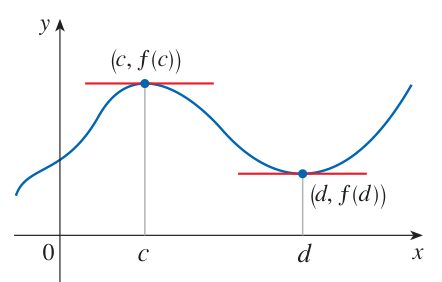
\includegraphics[width=\linewidth]{images/p0317_fig3.png}\\[3pt]
    {\footnotesize\textbf{\textsf{HÌNH 11}}}
  \end{minipage}\hspace{6mm}%
}%Nh
Hình 11 thể hiện đồ thị của một hàm số $f$ có cực đại địa phương tại $c$ và cực tiểu địa phương tại $d$. Có vẻ như tại các điểm cực đại và cực tiểu, các tiếp tuyến đều nằm ngang và do đó mỗi tiếp tuyến đều có hệ số góc bằng 0. Chúng ta biết rằng đạo hàm là hệ số góc của tiếp tuyến, vì vậy có vẻ như $f'(c) = 0$ và $f'(d) = 0$. Định lý sau đây khẳng định điều này luôn đúng đối với các hàm khả vi.

\vspace{0.6em}
\begin{tcolorbox}[
  colback=white,
  colframe=stewartred,
  arc=0mm,
  boxrule=0.7pt,
  left=3.5mm,
  right=3.5mm,
  top=2.5mm,
  bottom=2.5mm
]
  {\color{stewartred}\setlength{\fboxsep}{2pt}\fbox{\bfseries\textsf{\color{stewartred}4}}}\hspace{0.6em}%
  \textbf{\textsf{\color{stewartred}Định lý Fermat}}\hspace{1.2em}%
  Nếu $f$ có cực đại hoặc cực tiểu địa phương tại $c$, và nếu $f'(c)$ tồn tại, thì $f'(c) = 0$.
\end{tcolorbox}
\vspace{0.4em}

\noindent{\textbf{\textsf{\color{stewartred}CHỨNG MINH}}}\hspace{1em}%
Giả sử, để cho cụ thể, rằng $f$ đạt cực đại địa phương tại $c$. Khi đó, theo Định nghĩa 2, $f(c) \ge f(x)$ nếu $x$ đủ gần $c$. Điều này suy ra rằng nếu $h$ đủ gần 0, với $h$ là số dương hoặc âm, thì
\[
f(c) \ge f(c + h)
\]
và do đó
\vspace{-0.2em}
\noindent
\makebox[0pt][l]{\hspace{0.5em}{\color{stewartred}\setlength{\fboxsep}{2pt}\fbox{\bfseries\textsf{\color{stewartred}5}}}}%
\hfill $f(c + h) - f(c) \le 0$\hfill\null

\vfill
\noindent{\tiny\color{lightgray}%
Copyright 2021 Cengage Learning. All Rights Reserved. May not be copied, scanned, or duplicated, in whole or in part. Due to electronic rights, some third party content may be suppressed from the eBook and/or eChapter(s). Editorial review has deemed that any suppressed content does not materially affect the overall learning experience. Cengage Learning reserves the right to remove additional content at any time if subsequent rights restrictions require it.\par}
